\chapter{Discussion and Limitations}
\label{chap:discussion}

\section{Limitations}

This work presents a first attempt at analysing Wikipedia's edit filter system.
It has several limitations (we could think of).
First, it focuses on English Wikipedia only.
We are convinced that there are valuable lessons to be learnt (about the communities, usefulness of filters, ..) from comparing edit filter use across different language versions.
Second, unfortunately, including an ethnographic analysis was not possible.
This is partially due to the fact that we employ a computer science perspective on the question and partially due to limited time.
Third, the manual filter classification was undertaken by one person only, so biases of this person have certainly shaped the labels.

\section{Discussion}

* why get certain filters (and not others?)
* do filters solve effectively the task they were conjured up to life to fulfil?
* what kinds of biases/problems are there?
* who is allowed to edit edit filters?

Alternative approaches to community management:
compare with Surviving the Eternal September paper~\cite{KieMonHill2016}
"importance of strong
systems of norm enforcement made possible by leadership,
community engagement, and technology."

"emphasizing decentralized moderation" //all community members help enforce the norms
"ensuring enough leadership capacity is available
when an influx of newcomers is anticipated."
"Designers may
benefit by focusing on tools to let existing leaders bring others
on board and help them clearly communicate norms."
"designers should support an ecosystem of accessible and ap-
propriate moderator tools."


\subsection{The bigger picture: Upload filters}

The planned introduction of upload filters by the EU copyright reform is seen critically by Wikimedia Germany:
\begin{figure}
\centering
  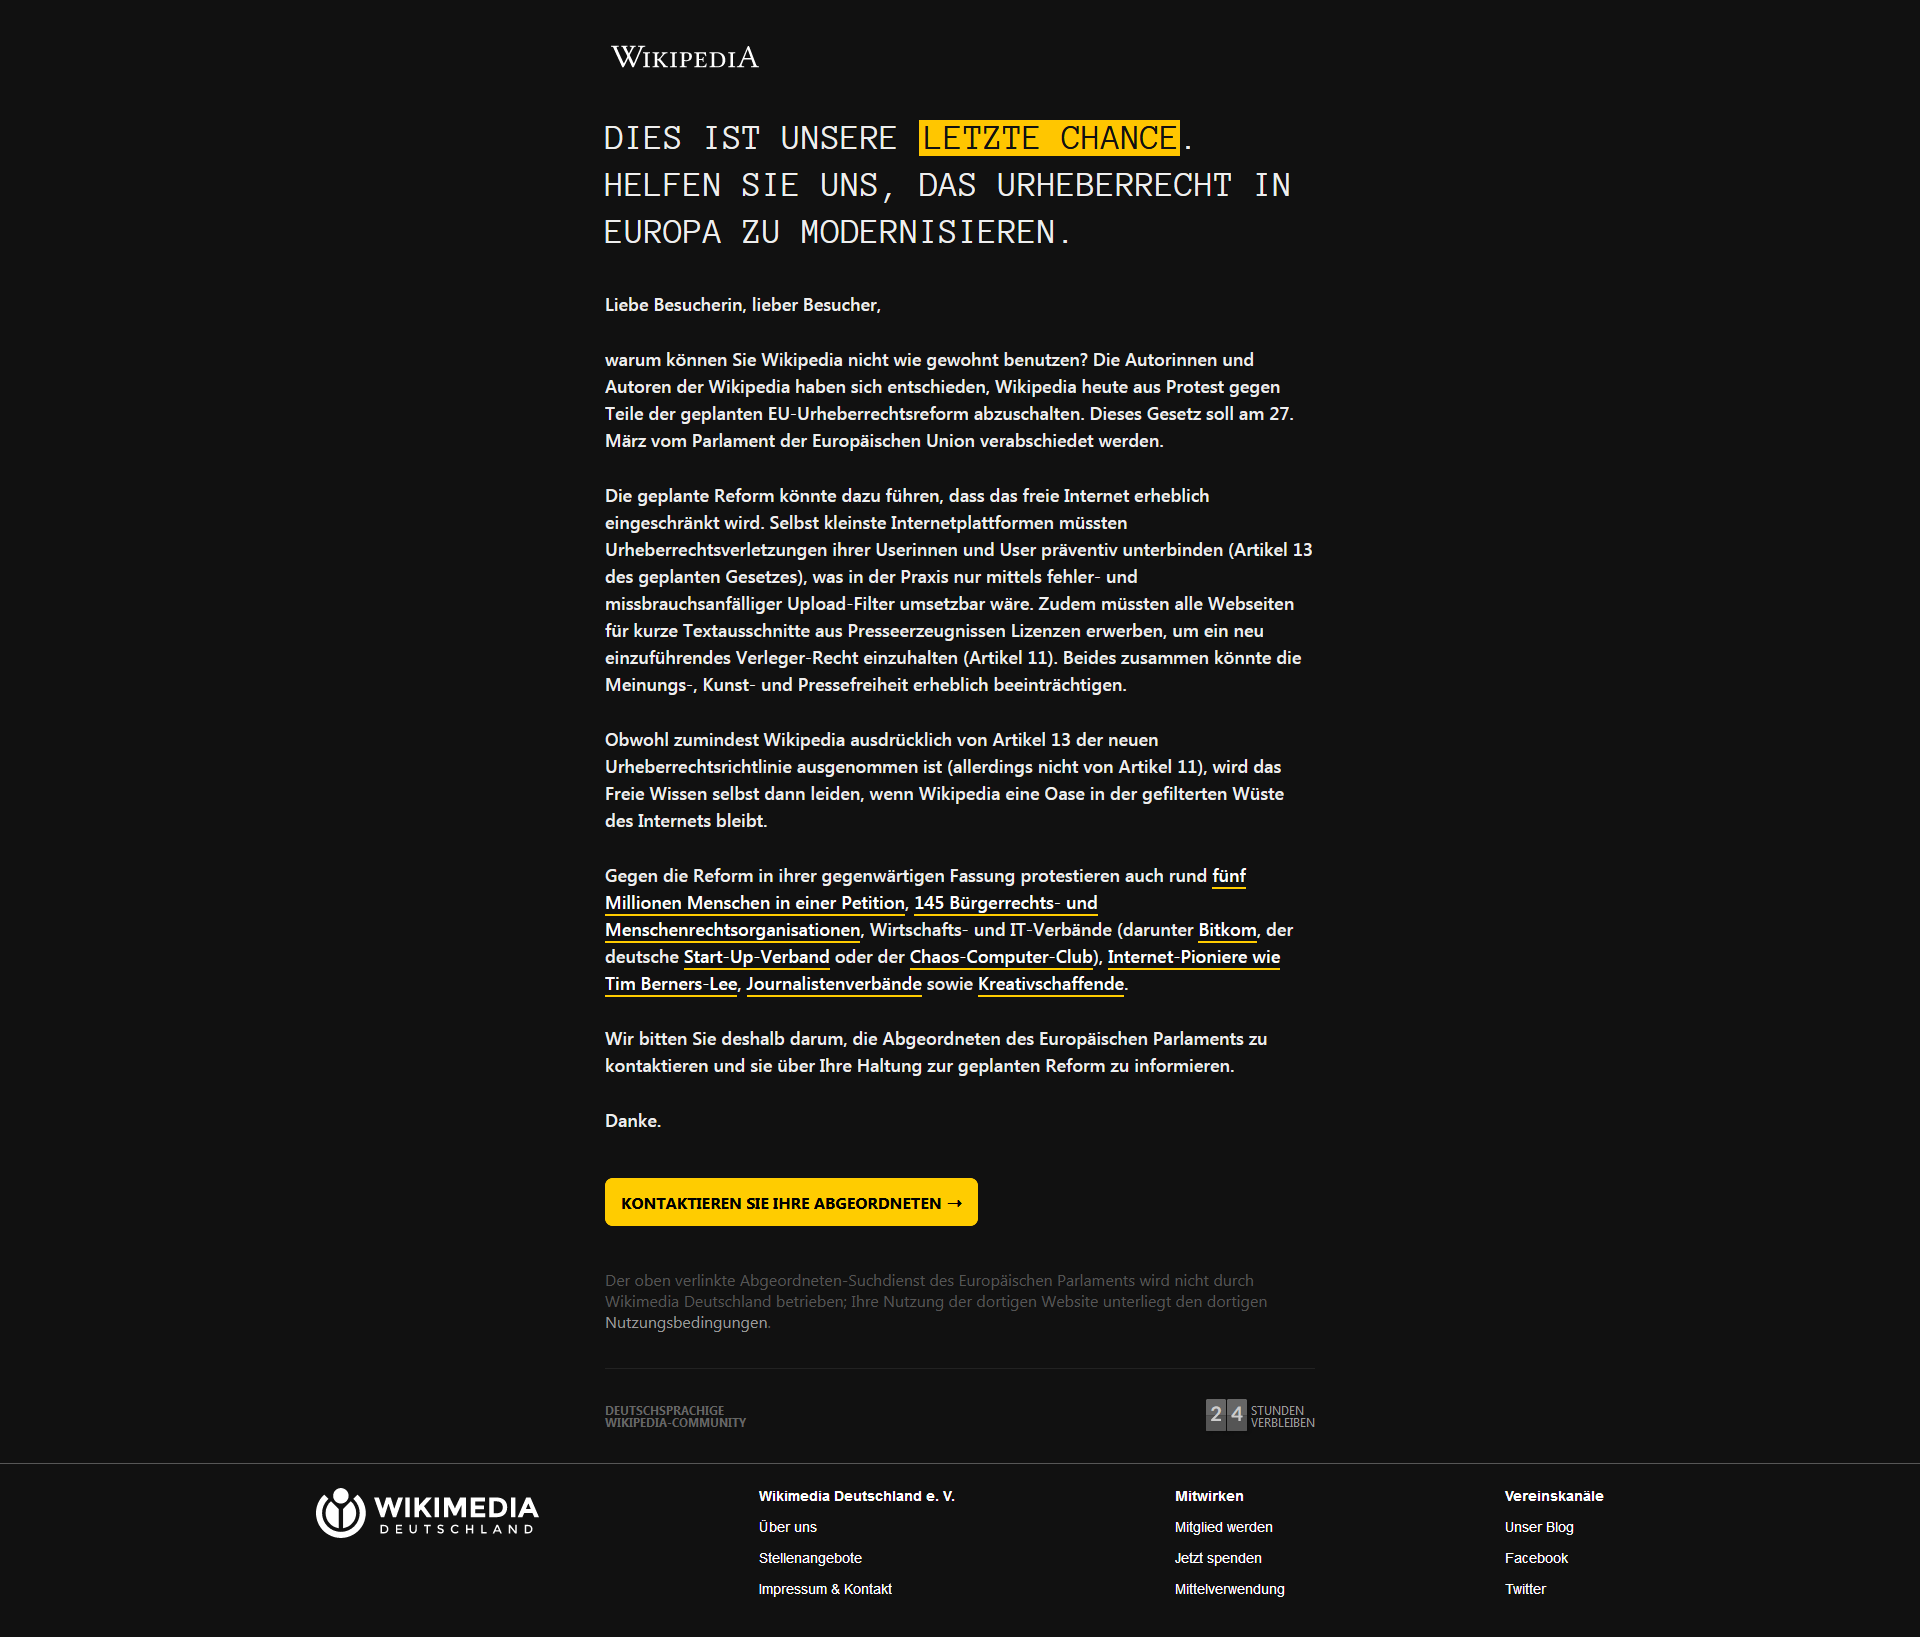
\includegraphics[width=0.9\columnwidth]{pics/Blackout_of_wikipediade_by_Wikimedia_Deutschland_-_March_2019.png}
  \caption{Blackout of wikipedia.de by Wikimedia Deutschland}~\label{fig:blackout-upload-filters}
\end{figure}

via
\url{https://de.wikipedia.org/wiki/Abschaltung_der_deutschsprachigen_Wikipedia_am_21._M%C3%A4rz_2019#/media/File:Blackout_of_wikipedia.de_by_Wikimedia_Deutschland_-_March_2019.png}

see also
\url{https://wikimediafoundation.org/2019/03/20/four-wikipedias-to-black-out-over-eu-copyright-directive/}
"Volunteer editor communities in four language Wikipedias—German, Czech, Danish, and Slovak—have decided to black out the sites on 21 March in opposition to the current version of the proposed EU Copyright Directive.

Those language editions of Wikipedia will redirect all visitors to a banner about the directive, blocking access to content on Wikipedia for 24 hours. "
"These independent language communities decided to black out in the same way most decisions are made on Wikipedia—through discussion and consensus, "

and
\url{https://wikimediafoundation.org/2019/02/28/we-do-not-support-the-eu-copyright-directive-in-its-current-form-heres-why-you-shouldnt-either/}

timeline
\url{https://edri.org/upload-filters-status-of-the-copyright-discussions-and-next-steps/}

\url{https://en.wikipedia.org/wiki/Directive_on_Copyright_in_the_Digital_Single_Market#Positions}

\subsection{Directions for further studies}
<insert long list of interesting questions here>
